\section{Playing Atari Games}

The aforementioned papers all use the Atari 2600 environment to train and test agent implementations.

We remark in the introduction chapter that \emph{original DQN} \cite{atari-dqn} study produced agents able to surpass human-level performance in \emph{Breakout}, \emph{Enduro} and \emph{Pong}.
The subsequent improvements to the original have of course managed to equal or surpass the original implementations \cite{ddqn-paper,per-paper}.

The \emph{Atari 2600 Learning Environment (ALE)} \cite{ale-paper} has become a popular benchmark used in the study of AI.
One of the reasons being that Atari games are often intuitive and fun to watch.
Researchers can often have a good measure of how well an agent behaves only by observing its performance on the Atari emulator.

\begin{figure}[]
    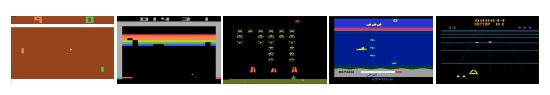
\includegraphics[width=\textwidth]{atari-screenshots}
    \centering
    \caption{Screen captures from different games on the Atari 2600 (Corresponds to fig. 1 in \cite{atari-dqn})}
    \label{fig:atari-games}
\end{figure}

\section{Roguelike Games}

\emph{Rogue} is a video game originally developed around 1980 for Unix-based mainframe system \cite{wiki:Rogue_(video_game)}.

\begin{figure}[]
    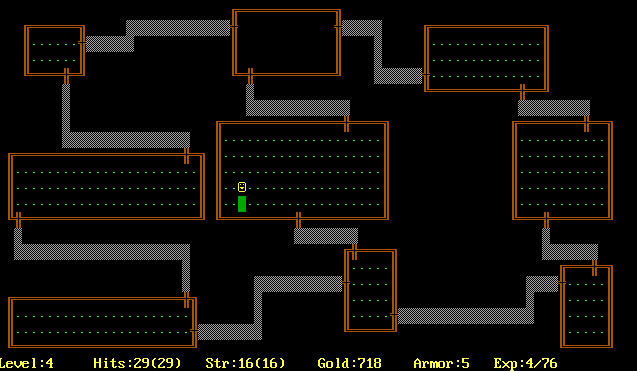
\includegraphics[width=0.75\textwidth]{rogue}
    \centering
    \caption{The iconic ASCII-based interface of rogue (from \cite{wiki:Rogue_(video_game)})}
    \label{fig:rogue}
\end{figure}

As a staple of the \emph{dungeon crawling} genre, the game requires the player to navigate \emph{dungeons}.
The layout of a dungeon is visible -- it consists of several rooms.
The player may start out in any one of them.
The exact position of every item, monster or door is unknown.
The game features exploration mechanics like searching for keys to open locked doors and hidden passages.

\emph{Rogue} would not be complete without its \emph{combat aspect}.
Although rudimentary, it was a fun, innovative mechanic for its time.
The game features monster encounters.
Monsters are visible to the player once they are close enough.
Their initial positions on a map are chosen at random and they have resistances that one has to find a way around and vulnerabilities that one can exploit.

An interesting feature, which distinguishes \emph{Rogue} from other adventure games of the era, is \emph{random generation}.
The game builds randomly-generated dungeon layouts and randomizes the placement of items and monsters inside it \cite{wiki:Rogue_(video_game)}.

Insipired by the simple yet fun qualities of this game, the genre of \emph{roguelikes} was born.
Part of this genre are games that enhance the original experience prodiving new mechanics or improving the original ones.
It is essentially a mix-match of the properties of the original game: random generation, one-life, enemy combat and item system.

We consider roguelikes to be an appropriate level of complexity for RL agents to handle and still thrive.
Rogue has the potential of creating interesting behaviour patterns which would help find and address problems in RL (and any specific method applied i.e. Q-learning).
One of the problems of RL is \textbf{generalization}:
an agent having developed a generalized skill is more useful than one which has simply managed to memorize its environment.
Rogue's randomly generated levels provide a good environment to test this.

There are studies using \emph{roguelikes} as an environment to study RL agents.
These studies aimed to train agents that produced optimal behaviour in environments closely matching the original game.
Below, we are going to present one case of significance.

In the \emph{Rogue-Gym} paper \cite{rogue-gym-paper}, researchers propose using Rogue as a benchmark for generalization.
As we mentioned above, one of Rogue's characteristics is random level generation.
This can be leveraged to study whether an agent has learned a skill or has just learned to retrace a certain environment.
In this paper, researchers use state-of-the-art policy optimization methods to train agents on a variant of Rogue without combat.
Its results are pointing out that most tested methods have poor generalization score.
This has to do both with Rogue's complexity as well as the shortcomings of the RL algorithms.